\section{Lucius III di Dishartha (Lucius Narendra
Pahaton)}\label{lucius-iii-di-dishartha-lucius-narendra-pahaton}

Tags: NPC Creatore: Lorenzo Luogo: Disharta, Goldendoor

\section{\texorpdfstring{\textbf{Lucius Narendra
Pahaton}}{Lucius Narendra Pahaton}}\label{lucius-narendra-pahaton}

\begin{center}\rule{0.5\linewidth}{0.5pt}\end{center}

\begin{figure}
\centering
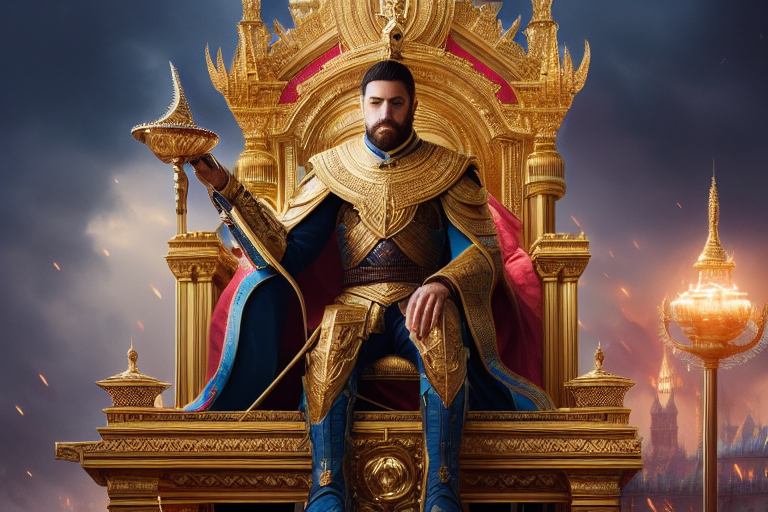
\includegraphics{01_IMPERATORE.png}
\caption{01\_IMPERATORE.png}
\end{figure}

Informazioni Generali

Età: 58

Data di nascita: 1996

Luogo di nascita: Goldendoor

Razza: Umano

Classe:

Alleati:

Nemesi:

Alias:

Professione: Imperatore di Disharta

\begin{center}\rule{0.5\linewidth}{0.5pt}\end{center}

\subsection{1. Descrizione Generale}\label{descrizione-generale}

\begin{center}\rule{0.5\linewidth}{0.5pt}\end{center}

\begin{figure}
\centering
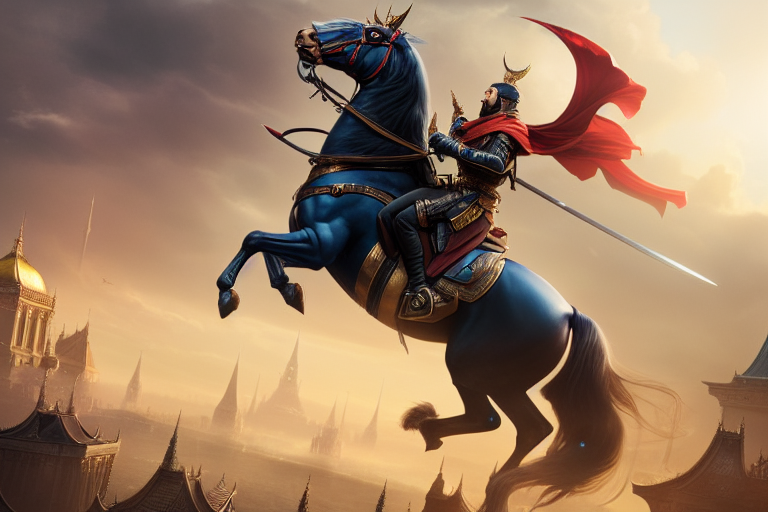
\includegraphics{emperor-on-his-trhone-trending-on-artstation-sharp-focus-studio-photo-intricate-details-highly-.png}
\caption{emperor-on-his-trhone-trending-on-artstation-sharp-focus-studio-photo-intricate-details-highly-.png}
\end{figure}

L'Imperatore Lucius III di Disharta è un uomo imponente con un
portamento regale. Ha capelli neriben pettinati e un viso severo con
occhi penetranti che riflettono la sua autorità. Indossa abiti sontuosi
e una corona d'oro che simboleggia la sua posizione di supremo sovrano.

\subsection{2. Biografia}\label{biografia}

\begin{center}\rule{0.5\linewidth}{0.5pt}\end{center}

Lucius III è nato nella famiglia reale di Disharta ed è cresciuto con
l'idea che un giorno avrebbe dovuto regnare sull'impero. È stato educato
nei principi della leadership, della politica e della strategia militare
fin dalla giovinezza. Ha salito i gradini della gerarchia reale fino a
diventare imperatore.

\subsection{3. Carriera}\label{carriera}

\begin{center}\rule{0.5\linewidth}{0.5pt}\end{center}

La carriera di Lucius III è stata dedicata al governo e alla gestione
dell'Impero di Disharta. Ha dimostrato di essere un sovrano abile,
maestro della diplomazia e dell'arte della politica. Ha guidato l'impero
attraverso periodi di prosperità e crisi, mantenendo la sua autorità
incondizionata. La sua preoccupazione principale è stata sempre
garantire la stabilità e la crescita dell'impero.

\subsection{4. Personalità}\label{personalituxe0}

\begin{center}\rule{0.5\linewidth}{0.5pt}\end{center}

L'Imperatore Lucius III è un uomo di ambizione ardente e determinazione
ferrea. Col passare degli anni, il suo unico desiderio è diventato
quello di assicurare la continuità del suo lignaggio e l'ascesa di un
erede maschio al trono di Disharta. Alla nascita della principessa Leona
il suo cuore è rimasto freddo, poiché la sua ambizione era rivolta a un
erede maschio. L'imperatore è noto per la sua freddezza e indifferenza
verso la figlia. Ha speso gran parte della vita della figlia a cercare
di forgiare alleanze matrimoniali per consolidare il suo potere,
ignorando le esigenze emotive di Leona. La sua decisione di cercare di
farla tornare al palazzo dopo la sua fuga è dettata più dalla
preoccupazione per la stabilità dell'impero che dall'affetto paterno.

\subsection{A. Coinvolgimenti in Eventi
Recenti}\label{a.-coinvolgimenti-in-eventi-recenti}

\begin{center}\rule{0.5\linewidth}{0.5pt}\end{center}

\href{Untitled\%20Database\%20665a498987254279b64261b8cc19c10e.csv}{Untitled
Database}
